\documentclass{icga}
\newif\iflong\longtrue
\newif\ifshort\shortfalse

\usepackage{graphicx}
\def\Eo{\mbox{\sc Ezo}}
\def\Hz{\mbox{\sc Hexamaze}}
\def\Mx{\mbox{\sc MoHex}}
\def\Mt{\mbox{\sc MoHexNet}}
\def\Nx{\mbox{\sc NeuroHex}}
\def\Sol{\mbox{\sc Solver}}
\def\Fuego{\mbox{\sc Fuego}}
\def\TV{\mbox{\sc TV}} %Tony van der Valk

\title{\sc ??? WINS HEX 11x11 and HEX 13x13 TOURNAMENTS}
\runningtitle{ICGA}
\author{Ryan Hayward\thanks{Department 
of Computing Science, University of Alberta, Canada. Email:hayward@ualberta.ca} and
Noah Weninger \thanks{CS, UAlberta, Email:nweninge@ualberta.ca} and
Kenny Young\thanks{CS, UAlberta. Email:kjyoung@ualberta.ca} and
Tony van der Valk\thanks{Email:tony@hexboard.com}
}
\affiliation{Edmonton, Canada}
\issue{???}

\setcounter{page}{999}
\begin{document}
\maketitle

\vspace*{-2.25in}
%{\it ICGA Journal Vol.\ XX No.\ YY Sept 999 pp ??-??
%\hfill Computer Games Olympiad, 2015 Leiden.}
{\it to appear, ICGA Journal}
\vspace*{2.0in}

\begin{figure}[hbt]
%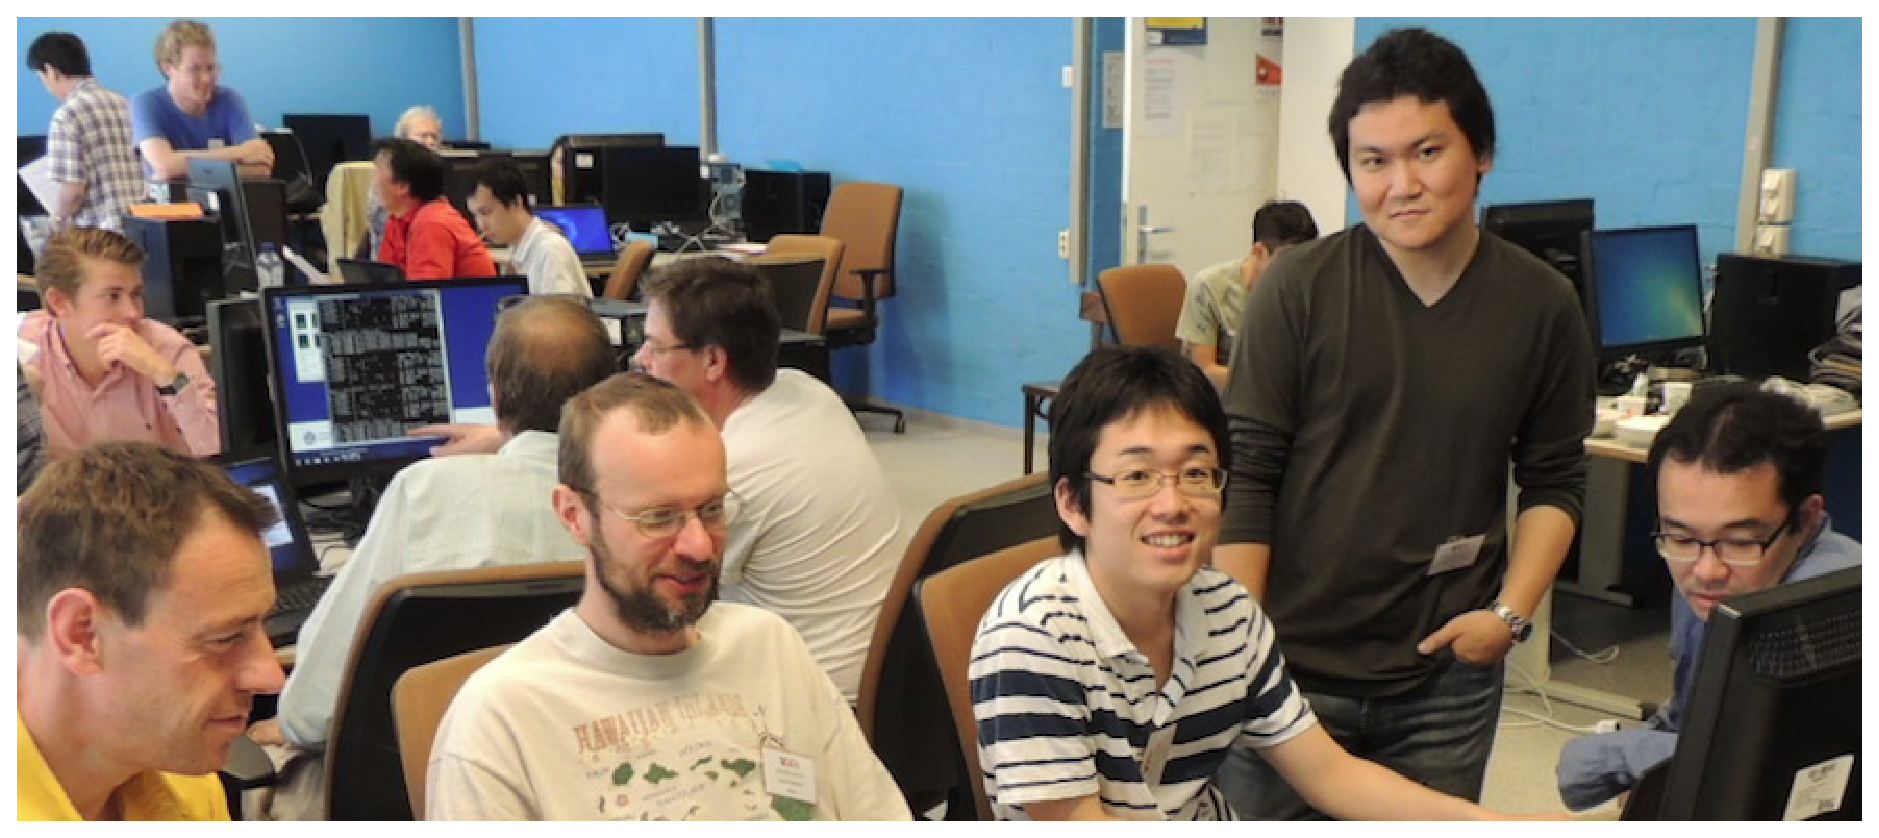
\includegraphics[width=225pt]{edo0.eps}\
%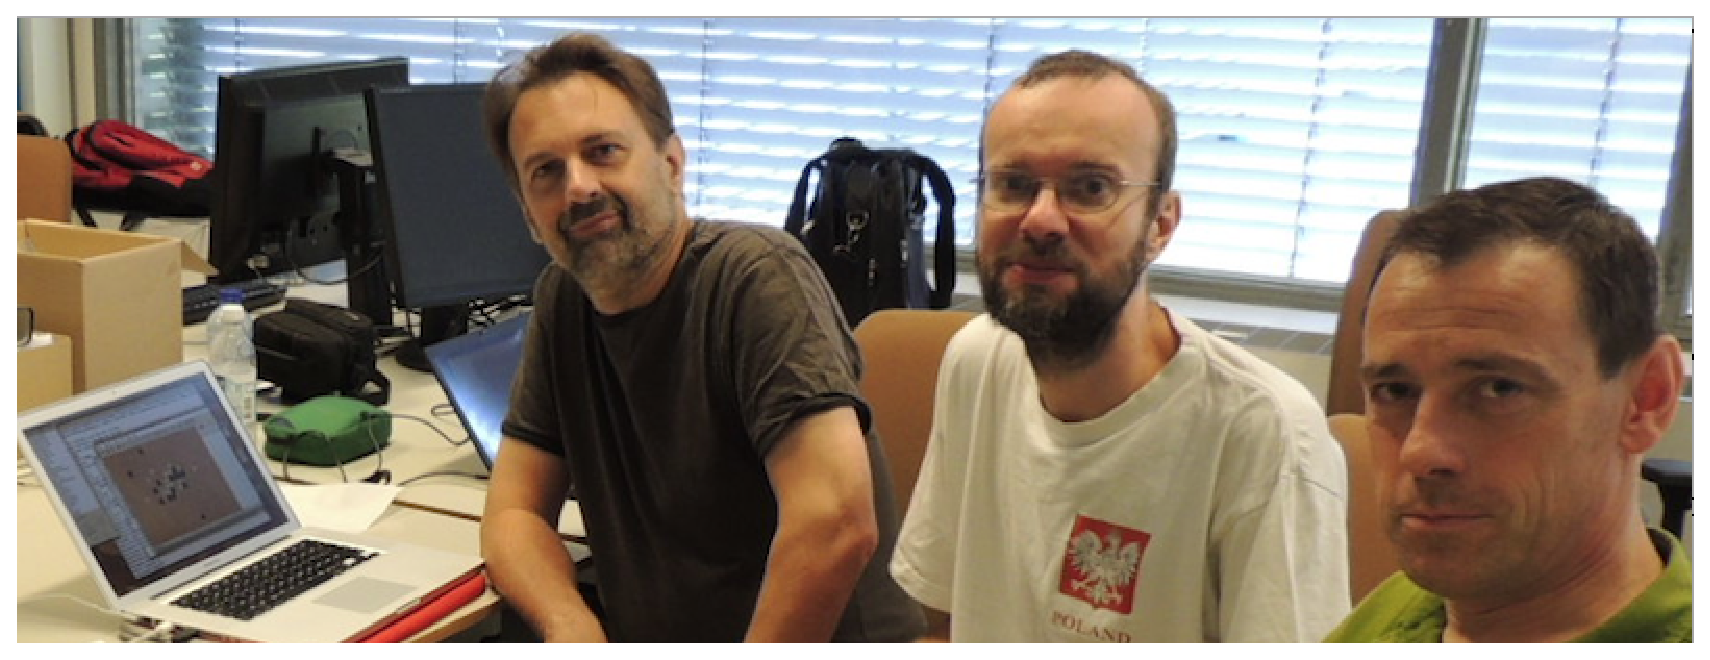
\includegraphics[width=225pt]{rjt2.eps}\\
TODO: new pix

%\hfill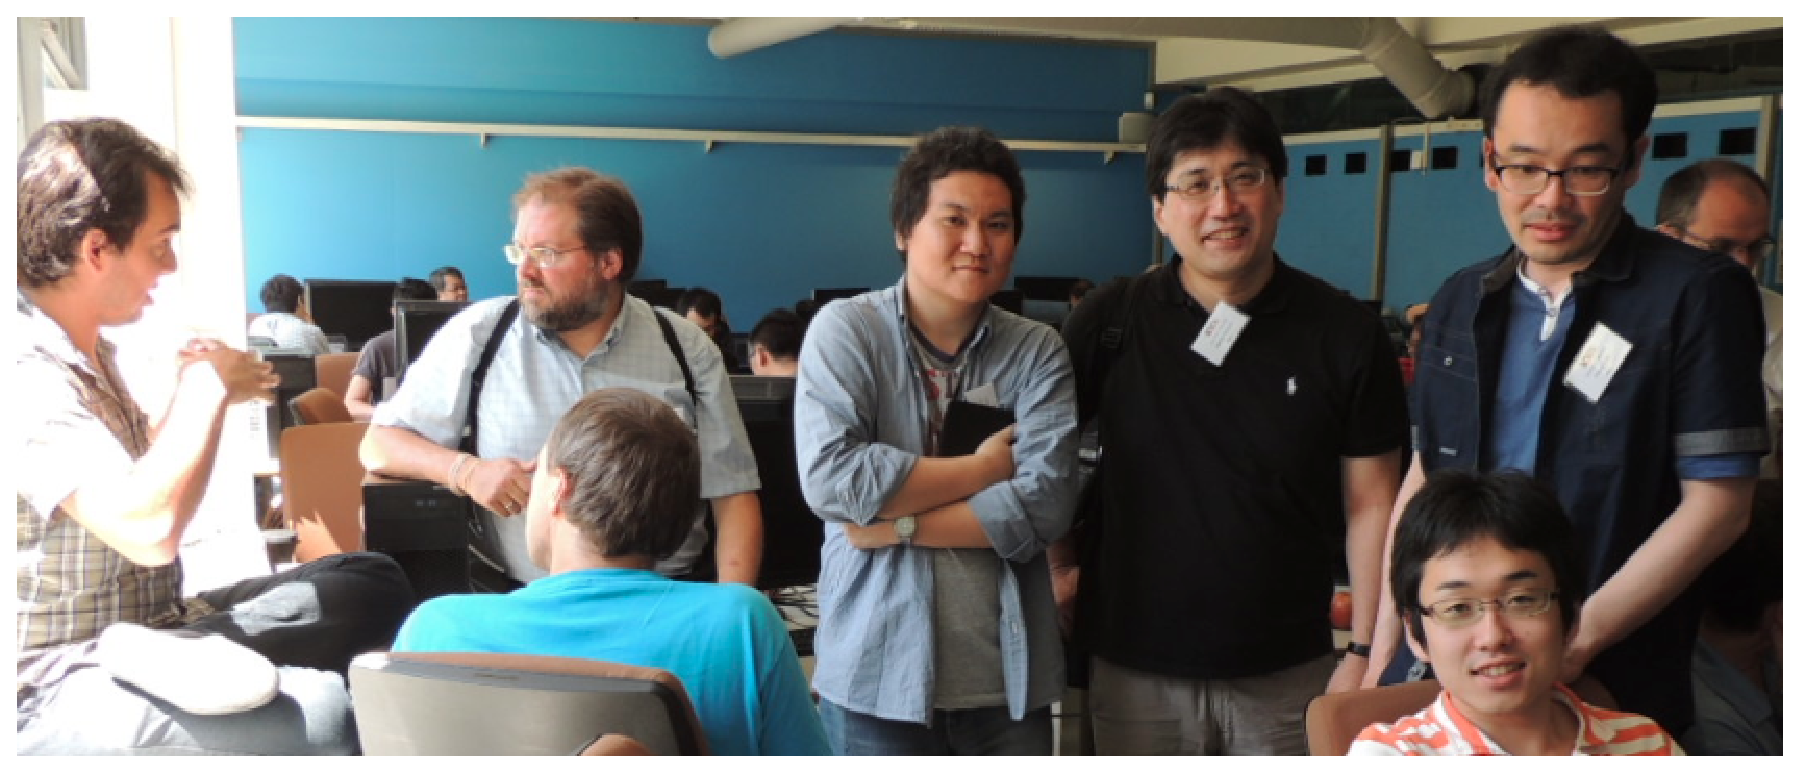
\includegraphics[width=280pt]{mas.eps}\hfill~
\caption{Participants and observers at the Hex competitions.}
\end{figure}


\section{The Tournaments}
At the 2016 Olympiad there were
two Hex tournaments: 11$\times$11 and 13$\times$13.
Three programs competed in the 11$\times$11 tournament:
\Eo{} by Kei Takada, supervised by Masahito Yamamoto, from Japan;
\Hz{} by Tianli Zhang, operated by Yunxiao Sun, from China; and
\Mx{} 2.0 \citebay{HAHMP13}, 
by Broderick Arneson, Ryan Hayward, Philip Henderson, Aja Huang, and Jakub Pawlewicz, from Canada.

Three programs competed in the 13$\times$13 tournament:
\Eo{}, \Hz{}, and \Mt{} from Canada,
with the same authors as \Mx{}, plus Noah Weninger and Kenny Young.

\Eo{} is a stronger version of the program that competed in the 2015 Olympiad.
\Eo{} is based on the Benzene framework and uses iterative deepening depth-first search with an evaluation function based on a weighted combination of some network connectivity measures.
\Eo{} ran on an i7 laptop and uses Benzene's 
Depth-First Proof Number Search solver.

\Hz{} is a new program?  by ?  

\Mx{}, the winner of the previous five Olympiad Hex competitions
\citebay{HAHP13},
is an MCTS program that uses the Benzene Hex framework
built on the code base of \Fuego\ \citebay{fuego},
the Go program developed by Martin M\"{u}ller, Markus Enzenberger
and others at the University of Alberta.
Benzene allows virtual connection and
inferior cell computations.
\Mx{} performs these computations in UCT tree nodes visited at least 256 times.
\Mx{} ran on a 24 core shared-memory machine, 
with 4 cores reserved for the 
Depth-First Proof Number Search solver, which
produces perfect play if it solves the
position within the time allotted for a move.
\Mx{} uses a book ---
built by Broderick Arneson using Thomas Lincke's method 
\citebay{DBLP:conf/cg/Lincke00} ---
with two 11$\times$11 openings.

\Mt{} is a new hybrid program that combines
the \Mx{} MCTS search tree with a 
depth-1 tree created by calling \Nx{}, 
a Deep Convolution Neural Net, once from the root.

TODO cite Nx paper.

Each tournament was a three-player double round robin, so 12 games
in total with 8 games per player.
Post-game win-detection is by our solver.
%Tony van der Walk contributed to this commentary.

{\large\bf 11$\times$11 Tournament}

\hfill\begin{tabular}{|c|c|c|c|c|c|}
\hline 11x11 results &\Mx{} &\Eo{} & \Hz{}     & total & result \\ 
\hline \Mx{} &      &  ?-?    &  ?-?      & ?-?  &  ? \\
\hline \Eo{} &  ?-? &  ?-?    &           & ?-?  &  ? \\
\hline \Hz{} &  ?-? &         &  ?-?      & ?-?  &  ? \\
\hline
\end{tabular}\hfill~

Here are some selected games.

{\bf Game 1.}
{\sc E-M 0-1.}
1.B[a7] 2.W[swap] 3.W[c9] \ldots ~ ~
\Mx{} sees the win by move 30.B[e4].

\begin{figure}[hbp]
\includegraphics[scale=1.3]{0556.eps}\hspace*{-1cm}\includegraphics[scale=1.3]{0556.eps}
\caption{Some game: \Eo-\Mx\ 0-1. Some game: }
\end{figure}

\newpage
{\large\bf 13$\times$13 Tournament}


\hfill\begin{tabular}{|c|c|c|c|c|c|}
\hline 13x13 results &\Mx{} &\Eo{}  &\Hz{}   & total & result \\ 
\hline \Mx{} &      &  ?-?    & ?-?  & bronze \\
\hline \Eo{} &  ?-? &  ?-?    & ?-?  & bronze \\
\hline \Hz{} &  ?-? &  ?-?    & ?-?  & bronze \\
\hline
\end{tabular}\hfill~

Above, playoff results are inside parentheses.
Here are some selected games.

\section{Conclusions}
%{\large\bf Conclusions}
%\Eo{}'s performance was stronger than its record indicates. 
%It played some strong openings and had winning moves deep
%into games against \Dx.
%It was unlucky not to win a game.

%\Dx\ and \Mx\ were evenly matched, but play different styles.
%\Mx\ seems stronger in opening and early middle play,
%but its Monte Carlo simulations cannot handle tactical positions.
%\Dx\ thrives on tactical positions, and is especially
%strong in the late middle game in complicated positions.

{\bf Acknowledgements.}
We thank the NSERC Discovery Grant Program for research funding and
Martin M\"{u}ller for the loan his machine.
\bibliography{rpt}
\end{document}
